\documentclass[tikz,border=5pt]{standalone}
\usetikzlibrary{positioning, arrows.meta, calc}
\usepackage{amsmath,amssymb}
\begin{document}
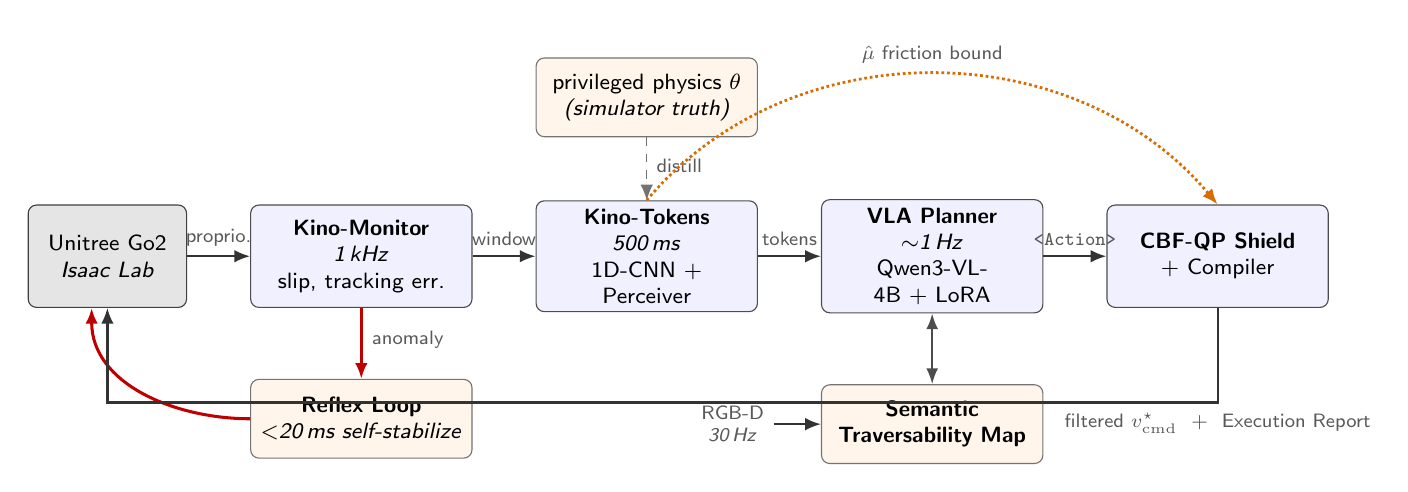
\begin{tikzpicture}[
  font=\sffamily\footnotesize,
  layer/.style={rectangle, rounded corners=3pt, draw=black!70, fill=blue!6,
                align=center, minimum height=13mm, text width=26mm, inner sep=3pt},
  plant/.style={rectangle, rounded corners=3pt, draw=black!75, fill=black!10,
                align=center, minimum height=13mm, text width=18mm, inner sep=3pt},
  aux/.style={rectangle, rounded corners=3pt, draw=black!55, fill=orange!8,
              align=center, minimum height=10mm, text width=26mm, inner sep=3pt},
  lab/.style={align=center, font=\sffamily\scriptsize, text=black!65},
  fwd/.style={-{Latex[length=2mm,width=1.6mm]}, thick, black!80},
  fast/.style={-{Latex[length=2mm,width=1.6mm]}, line width=1.1pt, red!75!black},
  distill/.style={-{Latex[length=2mm,width=1.6mm]}, dashed, black!55},
  couple/.style={-{Latex[length=2mm,width=1.6mm]}, densely dotted, line width=1pt, orange!85!black},
]
% main forward pipeline
\node[plant] (robot) {Unitree Go2\\\textit{Isaac Lab}};
\node[layer, right=8mm of robot] (mon) {\textbf{Kino-Monitor}\\\textit{1\,kHz}\\slip, tracking err.};
\node[layer, right=8mm of mon] (tok) {\textbf{Kino-Tokens}\\\textit{500\,ms}\\1D-CNN $+$ Perceiver};
\node[layer, right=8mm of tok] (vla) {\textbf{VLA Planner}\\\textit{$\sim$1\,Hz}\\Qwen3-VL-4B $+$ LoRA};
\node[layer, right=8mm of vla] (cbf) {\textbf{CBF-QP Shield}\\$+$ Compiler};

\draw[fwd] (robot) -- node[lab,above]{proprio.} (mon);
\draw[fwd] (mon) -- node[lab,above]{window} (tok);
\draw[fwd] (tok) -- node[lab,above]{tokens} (vla);
\draw[fwd] (vla) -- node[lab,above]{\texttt{<Action>}} (cbf);

% privileged distillation (training-time supervision)
\node[aux, above=8mm of tok] (theta) {privileged physics $\theta$\\\textit{(simulator truth)}};
\draw[distill] (theta) -- node[lab,right,pos=0.45]{distill} (tok);

% mu-hat coupling, over the top
\draw[couple] (tok.north) to[out=50,in=130] node[lab,above]{$\hat\mu$ friction bound} (cbf.north);

% reflex fast loop
\node[aux, below=9mm of mon] (reflex) {\textbf{Reflex Loop}\\\textit{$<$20\,ms self-stabilize}};
\draw[fast] (mon) -- node[lab,right,pos=0.45]{anomaly} (reflex);
\draw[fast] (reflex.west) to[out=180,in=-90] ([xshift=-2mm]robot.south);

% semantic map + RGB-D
\node[aux, below=9mm of vla] (map) {\textbf{Semantic}\\\textbf{Traversability Map}};
\draw[{Latex[length=2mm]}-{Latex[length=2mm]}, thick, black!70] (vla) -- (map);
\node[lab, left=6mm of map] (rgbd) {RGB-D\\\textit{30\,Hz}};
\draw[fwd] (rgbd) -- (map);

% big feedback loop: cbf -> robot
\draw[fwd] (cbf.south) -- ([yshift=-12mm]cbf.south)
  -- node[lab,below]{filtered $v_{\mathrm{cmd}}^{\star}$ \ $+$ \ Execution Report} ([yshift=-12mm]robot.south -| cbf.south)
  -- ([yshift=-12mm]robot.south)
  -- (robot.south);
\end{tikzpicture}
\end{document}
